\documentclass[../thesis.tex]{subfiles}

\begin{document}

\chapter{Модель сети} \label{chapter:model}

В этой главе представлено описание разработанной математической модели ПКС сети, описывающей динамику изменения счетчиков правил маршрутизации в сети с произвольной комбинацией установленных правил маршрутизации.
\\

ПКС сети предоставляют возможность анализировать текущее состояние сети при помощи счетчиков, установленных на правилах маршрутизации \cite{petrov2018mathematical, petrov2018forwarding}.
Счетчик каждого правила маршрутизации хранит информацию о количестве пакетов, которые были обработаны этим правилом с момента его установки на коммутатор.

Счетчики, установленные на коммутаторы, могут быть использованы для разработки алгоритма обнаружения скомпрометированных коммутаторов.
Основная идея алгоритма обнаружения заключается в том, что мы можем предсказывать значения счетчиков правил маршрутизации, основываясь на информации о сети, имеющейся на контроллере, и сравнивать их с реальными значениями.
Если значения отличаются, то в сети присутствует скомпрометированный коммутатор (глава \ref{chapter:algorithm}).

Задача предсказания значений счетчиков правил маршрутизации по набору выделенных счетчиков решается в \cite{tootoonchian2010opentm}.
Проблема заключается в том, что в этой статье задача предсказания рассматривается в сокращенной постановке --- предполагается, что для каждого сетевого потока установлены выделенные правила маршрутизации, то есть в сети отсутствуют сложные механизмы маршрутизации, такие как агрегация потоков или балансировка нагрузки.
Такая постановка не описывает случай сетей телеком операторов и центров обработки данных \cite{kreutz2015software}.

Таким образом, нужен алгоритм для предсказания счетчиков правил маршрутизации в сети с произвольной комбинацией установленных правил маршрутизации.
Для разработки такого алгоритма необходимо разработать математическую модель ПКС сети, которая будет описывать динамику изменения счетчиков правил маршрутизации.

К настоящему моменту существует несколько математических моделей ПКС сетей \cite{kazemian2012header, gutz2012splendid, khurshid2012veriflow, zakharov2014formal, yang2016real, kazemian2013real}.
Однако, одни модели нацелены на проверку сетевых политик и корректности протоколов \cite{gutz2012splendid, khurshid2012veriflow, zakharov2014formal, yang2016real}, в то время как другие нацелены на обнаружение ошибок администрирования сети, таких как циклы маршрутизации или нарушение связности сети, и решение проблем с изоляцией и утечкой трафика \cite{kazemian2012header, kazemian2013real}.
Ни одна из существующих моделей не описывают динамику изменения счетчиков правил маршрутизации.

В настоящей главе представлена математическая модель ПКС сети, работающей по протоколу OpenFlow \cite{openflow15}, описывающая значения счетчиков правил маршрутизации как потоковую функцию \cite{ford2015flows} на графе зависимостей правил \cite{kazemian2013real}.
В этой главе также описан алгоритм предсказания значений счетчиков правил маршрутизации.

\section{Граф зависимостей правил} \label{section:dependency_graph}

Для разработки алгоритма предсказания значений счетчиков правил маршрутизации необходимо разработать модель ПКС сети, которая описывает динамику сетевых потоков.
Разработанная модель представляет собой развитие существующих моделей ПКС, таких как \textit{Header Space Analysis} \cite{kazemian2012header} и графа зависимостей правил (\textit{Rule Dependency Graph}) \cite{kazemian2013real}. 

Основная идея модели \textit{Header Space Analysis} заключается в абстракции понятия заголовка пакета от конкретных протоколов, составляющих данный заголовок.
Пакеты представлены как точки некоторого пространства размерности $L$, где $L$ --- максимальный размер заголовка, а сетевые устройства представляются функциями, заданными на том же пространстве.

Основной идеей графа зависимостей правил является то, что в модельном графе сети вершинами являются не сетевые устройства, а конкретные правила маршрутизации, установленные на данные сетевые устройства.
Ребрами в модельном графе являются возможные переходы пакетов между правилами маршрутизации.

Представление сети в виде графа зависимостей правил позволяет описывать произвольные комбинации правил маршрутизации, установленные в сети.
Таким образом, возможно описание как сложных механизмов маршрутизации (агрегация потоков и балансировка нагрузки), так и ошибок маршрутизации (конечные циклы маршрутизации).

Для разработанной модели ПКС сети доказано правило прохождения потока через вершины графа зависимостей правил и показано, как эта модель может быть использована для разработки алгоритма предсказания значений счетчиков правил маршрутизации.
Также в этой главе строго формализуется и расширяется модель \textit{Rule Dependency Graph}, которая была впервые неформально описана в \cite{kazemian2013real}.
\\

\subsection{Пространство заголовков}

В этой главе представлено подробное описание модели \textit{Header Space Analysis} \cite{kazemian2012header}.
\\

\textit{Пространством заголовков} пакетов называется множество $\mathcal{H}$, состоящее из векторов $h\in \{0,1\}^L$, где $L$ --- верхняя граница длины заголовков пакетов.

\textit{Сетевым пространством} называется множество $\mathcal{N}$, являющееся декартовым произведением $\mathcal{H} \times \mathcal{P}$, где $\mathcal{P}$ --- множество портов всех коммутаторов.
Это пространство представляет собой все возможные заголовки пакетов, находящиеся на всех возможных портах коммутаторов.
\textit{Сетевым пространством коммутатора} $W$ назовем множество $\mathcal{N}_W = \mathcal{H} \times \mathcal{P}_W \subseteq \mathcal{N}$, где $\mathcal{N}$ --- сетевое пространство.
Это пространство представляет собой все возможные заголовки пакетов, проходящих через порты коммутатора $W$.
Любое подмножество $D\subseteq \mathcal{N}$ будем называть \textit{доменом}.

\textit{Передаточной функцией коммутатора} $W$ назовем функцию $T_S:\ \mathcal{N} \rightarrow 2^{\mathcal{N}}$, которая моделирует работу коммутатора $W$ по обработке пакетов.
\begin{equation}
T_W(h,p) = \big\{ (h_1,p_1), (h_2,p_2), \dots, (h_k,p_k) \big\},
\end{equation}
где $p_1,p_2,\dots,p_k\in \mathcal{P}_W$.
Необходимо отметить, что пары $(h_i,p_i)$ не обязательно должны быть различными, т.е. значением функции $T_W(h,p)$ является мультимножество \cite{jech2013set}.

\textit{Сужением передаточной функции $T_W$ на порт $r\in \mathcal{P}_W$} назовем следующую функцию:
\begin{equation}
T^r_W(h,p) = \big\{ (h',r)\ |\ (h',r)\in T_W(h,p) \big\}.
\end{equation}

Таким образом, передаточную функцию можно представить следующим образом:
\begin{equation}
  T_W(h,p) = \bigcup_{r\in \mathcal{P}_W} {T^r_W(h,p)}.
\end{equation}

\textit{Доменом $D_{T_W}$ передаточной функции $T_W$} называется множество всевозможных пар $(h,p)$, которые принимаются этой функцией в качестве аргументов и не отображаются в пустое множество.
То есть:
\begin{equation}
D_{T_W} = \big\{ (h,p)\ |\ T_W(h,p)\neq \varnothing \big\}.
\end{equation}

Для передаточной функции $T_W$ каждого коммутатора определена \textit{обратная функция} $T^{-1}_W:\mathcal{N} \rightarrow 2^{\mathcal{N}}$ следующего вида:
\begin{equation}
T^{-1}_W(h,p) = \big\{ (h',p')\ |\ (h,p)\in T_W(h',p') \big\}.
\end{equation}

\textit{Сетевой передаточной функцией} называется функция $\Psi:\mathcal{N} \rightarrow 2^{\mathcal{N}}$, которая представляет собой композицию всех передаточных функций и моделирует работу всех коммутаторов.
\begin{equation}
\Psi(h,p) = 
\begin{cases}
    T_{W_1}(h,p),& \text{если } p\in W_1,\\
    \dots\\
    T_{W_n}(h,p),& \text{если } p\in W_n.
\end{cases}
\end{equation}

\textit{Топологической передаточной функцией} называется функция $\Gamma:\mathcal{N} \rightarrow \mathcal{N}$, которая моделирует поведение каналов связи, передающих пакеты с порта одного устройства на порт другого.
\begin{equation}
\Gamma(h,p) = 
\begin{cases}
    \big\{ (h,p^*) \big\},& \text{если } p \textit{ соединен с } p^*, \\
    \big\{ (h,p) \big\},& \text{если } p \textit{ не соединен}.
\end{cases}
\end{equation}

Используя приведенные выше передаточные функции, возможно смоделировать поведение пакета, который проходит некоторый путь в сети, применяя на каждом сетевом устройстве, находящемся на пути следования пакета, функцию $\Phi(h,p) = \Gamma(\Psi(h,p))$.
Например, если пакет с заголовком $h$ приходит на некоторый порт $p$, то его заголовок после прохождения $k$ коммутаторов будет равен
\begin{equation}
\Gamma\bigg(\Psi\Big(\dots\Gamma\big(\Psi(h,p)\dots\big)\Big)\bigg),
\end{equation}
или более кратко $\Phi^k(h,p)$.

\begin{comment}
\subsection{Представление множеств}

Для задания множеств в пространстве заголовков используются \textit{wildcard} маски.
Каждая \textit{wildcard} маска это последовательность $L$ символов $0$, $1$ или $x$, где $x$ описывает произвольный элемент.
Каждое множество в пространстве заголовков может быть представлено в виде набора \textit{wildcard} масок.
Например множество:
\begin{equation} \label{eq:exampleset}
H = \{000, 001, 010, 011, 100, 101, 110\}
\end{equation}
может быть представлено в виде $0xx + 10x + 110$.
Сумма \textit{wildcard} масок описывает объединение множеств, описываемых каждой отдельной маской.

Стоит отметить, что множество \eqref{eq:exampleset} также может быть представлено как разность \textit{wildcard} масок $xxx - 111$.
Разность \textit{wildcard} масок в данном случае описывает разность множеств, соответствующих этим маскам.
Введение операции разности \textit{wildcard} масок позволяет создавать более компактные представления доменов в модели \textit{Header Space} \cite{petrov2018forwarding}.

\begin{definition}
\textit{wildcard} выражением $W$ назовем выражение следующего вида:
\begin{equation} \label{eq:wildcard_expression}
W = \sum_{i\in[1,n]} {\big(x_i - \sum_{j\in[1,m_i]} {y_{ij}}\big)}
\end{equation}
Где $x_i$ и $y_{ij}$ --- \textit{wildcard} маски, и $y_{ij}\subseteq x_i$ для любого $i\in [1,n]$ и для любого $j\in[1,m_i]$.
Под операцией включения $\subseteq$ понимается включение множеств, описываемых \textit{wildcard} масками.
Маски $x_i$ далее будем называть \textit{положительными}, а маски $y_{ij}$ --- \textit{отрицательными}.
\end{definition}

Каждое множество $H$ в пространстве $\mathcal{H}$ может быть представлен в виде \textit{wildcard} выражения.
В качестве примера такого выражения можно привести:
\begin{equation}
\begin{split}
W & = \big(1xxx0 - (11x10 + 101x0)\big)\\
& + \big(0xxxx - (0xx1x + 0xxx0)\big)\\
& + \big(1xx11 - (10x11)\big)
\end{split}
\end{equation}
которое описывает множество:
\begin{equation}
\begin{split}
H & = \big\{10001, 10010, 11000, 11100, 00001,\\
& \ \ \ \ \ \ 00101, 01001, 01101, 11011, 11111 \big\}
\end{split}
\end{equation}

Для того, чтобы работать с описанной выше моделью, необходимо ввести теоретико-множественные операции над \textit{wildcard} выражениями, описывающими множества в пространстве заголовков. Далее под $x^k_i$ и $y^k_{ij}$  будем обозначать положительные и отрицательные элементы \textit{wildcard} выражения $W_k$.

\textit{Объединением} \textit{wildcard} выражений $W_1$ и $W_2$ называется \textit{wildcard} выражение $W_1\cup W_2$ вида:
\begin{equation}
W_1\cup W_2 = \sum_{i\in[1,n_1]} {\big(x^1_i - \sum_{j\in[1,m^1_i]} {y^1_{ij}}\big)} + \sum_{i\in[1,n_2]} {\big(x^2_i - \sum_{j\in[1,m^2_i]} {y^2_{ij}}\big)}
\end{equation}

\textit{Пересечением} \textit{wildcard} выражений $W_1$ и $W_2$ называется \textit{wildcard} выражение $W_1\cup W_2$ вида:
\begin{equation}
W_1\cap W_2 = 
\end{equation}

\textit{Дополнением} \textit{wildcard} выражения $W$ называется \textit{wildcard} выражение $\overline{W}$ вида:
\begin{equation}
\overline{W} = 
\end{equation}

\textit{Разницей} \textit{wildcard} выражений $W_1$ и $W_2$ называется \textit{wildcard} выражение $W_1 - W_2$ вида:
\begin{equation}
W_1 - W_2 = W_1\cap \overline{W_2}
\end{equation}
\end{comment}

\subsection{Формализация графа зависимостей правил}

В этой главе представлена строгая формализация и расширение существующей модели ПКС, называемой \textit{графом зависимостей правил} \cite{kazemian2013real}.
Расширение модели заключается в возможности описания множественных таблиц маршрутизации, групповых правил и набора различных действий, производимых правилами маршрутизации.

\textit{Графом зависимостей правил} назовем ориентированный граф $G=$\linebreak$G(V,A)$, где $V$ --- множество вершин, и $A$ --- множество ориентированных ребер.
Множество вершин $V$ графа $G$ построим следующим образом.

Для каждого правила маршрутизации, установленного в сети, добавим в множество $V$ вершину $v$.
Для каждого группового правила маршрутизации, добавим вершины $g,b_1,\dots,b_k$, где $k$ --- количество \textit{bucket}-записей \cite{openflow15} этого группового правила.
\textit{bucket}-записи описывают действия над копиями пакета, которые производят групповые правила маршрутизации.

Для каждого порта $p\in\mathcal{P}$ добавим в множество $V$ пару вершин $s$ и $t$, называемых \textit{источником} и \textit{стоком порта} $p$.
Эти вершины описывают клиентов, подключенных к коммутаторам.
Также, добавим в множество $V$ два выделенных стока $c$ и $d$, которые будем называть \textit{контроллером} и \textit{сбросом}.
Множества всех источников и стоков в графе $G$ будем обозначать как $S$ и $T$ соответственно.
Будем считать, что $S\neq \varnothing$, $T\neq \varnothing$ и $V\setminus (S\cup T)\neq \varnothing$.

\begin{figure}
\centering
\begin{subfigure}[b]{0.45\textwidth}
  \centering
  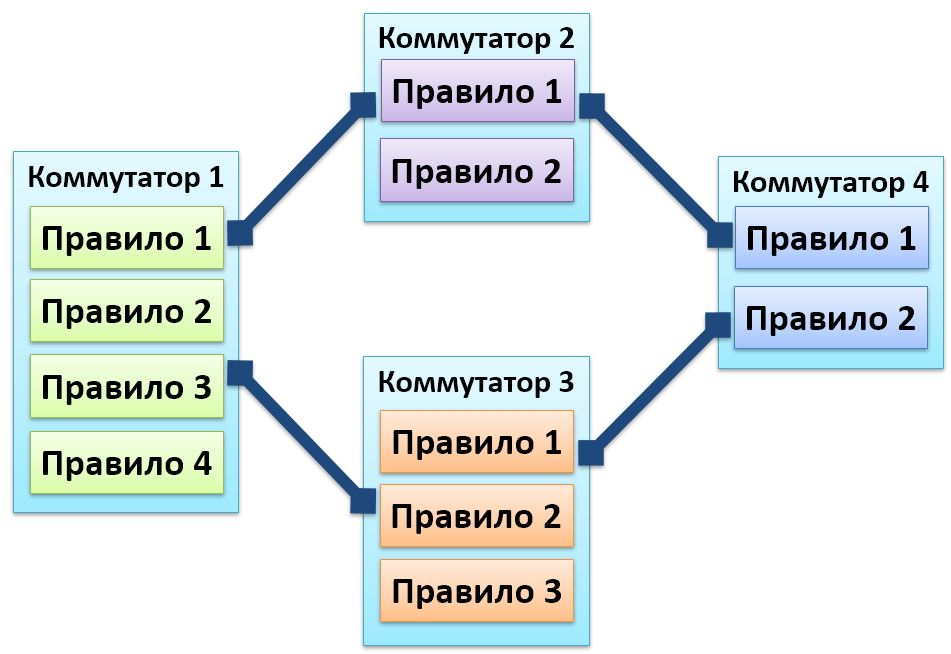
\includegraphics[width=0.95\textwidth]{figures/switchrules.jpg}
  \caption{Топология сети} \label{fig:switchrules}
\end{subfigure}
\begin{subfigure}[b]{0.45\textwidth}
  \centering
  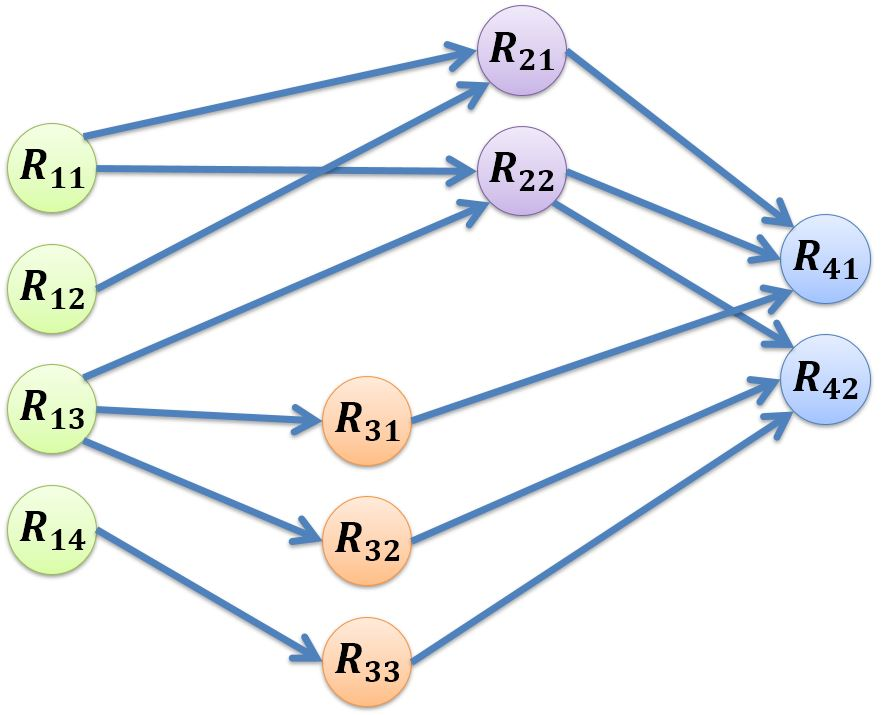
\includegraphics[width=0.85\textwidth]{figures/dependencygraph.jpg}
  \caption{Граф зависимостей правил} \label{fig:dependencygraph}
\end{subfigure}
\caption{Построение графа зависимостей правил}
\end{figure}

Далее, когда будем говорить “вершина $v$”, то будем подразумевать вершину $v\in V$, а когда будем говорить “правило $v$”, будем подразумевать правило маршрутизации, которому соответствует вершина $v$.

Каждой вершине $v\in V$ поставим в соответствие \textit{передаточную функцию} $T_v:\mathcal{N} \rightarrow 2^{\mathcal{N}}$:
\begin{equation} \label{eq:transfer}
    T_v(n) = \big\{ n_1,n_2,\dots,n_{\gamma(v)} \big\},
\end{equation}
где $n,n_1,\dots,n_{\gamma(v)}\in \mathcal{N}$.
Передаточная функция $T_v$ моделирует работу правила $v$ по обработке пакетов.
Если вершина $v$ является истоком или стоком, то передаточная функция $T_v$ единична, то есть $T_v(n) = \{n\}$.
Число $\gamma=\gamma(v)$ называется \textit{степенью дублирования вершины $v$}.

\textit{Доменом} $D_{T_v}$ \textit{передаточной функции} $T_v$ назовем множество всех доменов $n$, которые не преобразуются передаточной функцией в пустое множество:
\begin{equation} \label{eq:transfer_domain}
    D_{T_v}
    =
    \big\{ n\ |\ T_v(n)\neq \varnothing \big\}.
\end{equation}
Домен $D_{T_v}$ описывает поле \textit{match} правила $v$, то есть множество пакетов, которые обрабатываются этим правилом.
\\

Необходимо отметить, что $\big|T_v(n)\big| = \gamma(v)\ \ \forall n\in \mathcal{N}$, то есть степень дублирования фиксирована для каждой вершины, потому что значения $n_i$ на выходе передаточной функции описывают список действий (\textit{OpenFlow action list} \cite{openflow15}), который правило $v$ выполняет при обработке пакета.

\textit{Дублирующим правилом} назовем такое правило $v$, что существует домен $n\in \mathcal{N}$ такой, что $\gamma(v) > 1$.
Истоки $s\in S$ и стоки $t\in T$ не являются дублирующими вершинами по определению.

Также для каждой вершины $v\in V$ определим \textit{обратную передаточную функцию} $T^{-1}_v:\mathcal{N} \rightarrow 2^{\mathcal{N}}$:
\begin{equation} \label{eq:inverse_transfer}
    T^{-1}_v(n)
    =
    \big\{ n'\ |\ n\in T_v(n') \big\}.
\end{equation}

Каждой вершине $v$, не являющейся истоком, стоком, группой или \textit{bucket}-\linebreak записью, поставим в соответствие натуральное число $pr_v$, называемое \textit{приоритетом} данной вершины.
Определим на множестве вершин $V$ отношение частичного порядка <<$\succ$>> следующим образом:
\begin{equation} \label{eq:partial_order}
    v \succ u
    \Leftarrow
    \begin{cases}
        pr_v > pr_u,\\
        v,u\in V_{\tau},
    \end{cases}
\end{equation}
где $V_{\tau}$ --- множество вершин, соответствующих правилам в таблице $\tau$.
То есть вершины сравнимы, если они соответствуют правилам из одной таблицы.

Приоритет вершины $v$ описывает поле \textit{priority} правила маршрутизации, соответствующего этой вершине.
Таким образом, описанное отношение частичного порядка представляет собой очередность, в которой проверяется, какое правило должно обработать некоторый пакет.
Например, пакет с заголовком $h$, поступивший на порт $p$ коммутатора $S$, будет обработан максимально приоритетным правилом $v$ данного коммутатора таким, что $(h,p)\in D_{T_v}$.

Протокол OpenFlow описывает, что наличие правил с одинаковым приоритетом и пересекающимися доменами ведет к неопределенному поведению \cite{openflow15}.
Поэтому, мы можем предположить, что домены правил, имеющих одинаковый приоритет, не пересекаются.

Каждой вершине $v$ поставим в соответствие множество $D_{v}\subseteq \mathcal{N}$, называемое \textit{доменом вершины} $v$.
Под доменом вершины $v$ понимается множество заголовков пакетов, которые могут быть обработаны этим правилом с учетом приоритета, то есть:

\begin{equation} \label{eq:vertex_domain}
    D_{v}
    =
    D_{T_v} \setminus \bigcup_{w\succ v} {D_{T_w}}.
\end{equation}

Множество заголовков пакетов может измениться после обработки правилом $v$, так как в своей работе правило $v$ может изменять заголовок некоторого пакета, тем самым получая новый пакет.
Например, пусть правило $v$ обрабатывает пакеты с некоторой парой $\langle IP_{src},IP_{dst}\rangle$ с любого порта, устанавливает для таких пакетов некоторый \textit{VLAN ID} \cite{thaler2013ieee} и отправляет на порт $p'$.
Тогда доменом $D_v$ этой вершины будут все пары $(h,p)$, где $h$ --- заголовки пакетов с соответствующими значениями \textit{IP} адреса источника и получателя, а $p$ --- все порты коммутатора, на котором установлено правило $v$.
Множество $T_v(D_v)$ будет состоять из всех пар $(h',p')$, где $h'$ --- заголовки из $D_v$ с установленным \textit{VLAN ID}.

Пусть вершина $v\in S\cup T$, то есть является либо истоком, либо стоком некоторого порта $p$.
Поставим этой вершине в соответствие домен, равный $\mathcal{N}_p=\mathcal{H}\times p$, то есть всему сетевому пространству порта $p$.
Контроллеру $c$ и стоку $d$ поставим в соответствие домен $\mathcal{N}$, описывающий все сетевое пространство.

Множество ориентированных ребер $A$ графа $G$ построим следующим образом.

Пусть некоторая вершина $v$ отправляет пакеты в таблицу $\tau$.
Тогда соединим вершину $v$ ребрами с каждой вершиной $w\in V_{\tau}$.
Если вершина $v$ отправляет пакеты в групповое правило маршрутизации, которое соответствует вершинам $g,b_1,\dots,b_k$, добавим ребро $vg$.
Также, для каждого группового правила добавим ребра $gb_i$ для каждого $i\in [1,k]$.

Если порт $p$ подключен к некоторому порту $p^*$ физической линией, то соединим вершину $v$ ребрами с каждой вершиной $w\in V_{\tau_0}$, где $\tau_0$ --- нулевая таблица коммутатора, содержащего порт $p^*$.
Если порт $p$ не подключен, то добавим ребро $vt$, где $t$ --- сток порта $p$.
Если правило отправляет пакеты на контроллер или сбрасывает, то добавим ребра $vc$ и $vd$ соответственно.

Исток $s$ каждого порта $p$, не соединенного физической линией с другим портом сети, соединим ребрами со всеми правилами $w\in V_{\tau_0}$, где $\tau_0$ --- нулевая таблица коммутатора, содержащего порт $p$.

Ребра графа зависимостей правил показывают возможные пути следования пакетов между правилами маршрутизации (рис. \ref{fig:edges}). То есть, если существует ребро $a=vw$, это значит, что существуют пакеты, которые после обработки правилом $v$ будут обработаны правилом $w$.

\begin{figure}
\centering
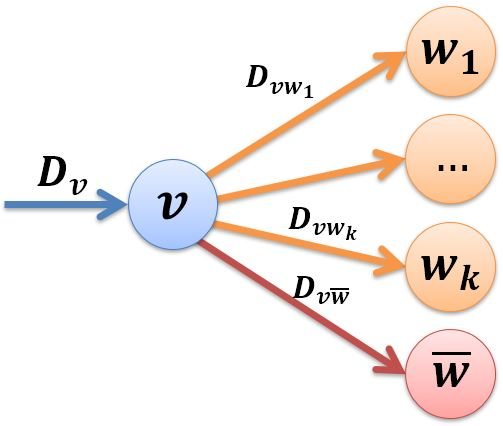
\includegraphics[width=0.4\textwidth]{figures/edges.jpg}
\caption{Ребра графа зависимостей правил} \label{fig:edges}
\end{figure}

Каждой вершине $v\in V$ поставим в соответствие \textit{сетевую передаточную функцию} $\Phi_v:\mathcal{N} \rightarrow 2^{\mathcal{N}}$.
Эта функция моделирует модификацию доменов при прохождении через вершину $v$ в графе зависимостей правил.
Если $T_v(n) = \big\{ n_1,n_2,\dots,n_{\gamma(v)} \big\}$ и $n_i = (h_i,p_i)$, где $h_i$ --- заголовок, а $p_i$ --- порт, то:
\begin{equation} \label{eq:network_transfer}
    \Phi_v(n)
    =
    \big\{ (h_1,p^*_1),(h_2,p^*_2),\dots,(h_{\gamma(v)},p^*_{\gamma(v)})\big\},
\end{equation}
где $p^*_i$ --- порт, соединенный с портом $p_i$, если функция $T_v$ отправляет домен $n_i$ на порт $p_i$.
Если же пакеты отправляются в некоторую таблицу маршрутизации, групповое правило, сбрасываются или отправляются на контроллер, то $p^*_i = p_i$.

Также каждой вершине $v\in V$ поставим в соответствие \textit{обратную сетевую передаточную функцию} $\Phi^{-1}_v:\mathcal{N} \rightarrow 2^{\mathcal{N}}$:
\begin{equation} \label{eq:inverse_network_transfer}
    \Phi^{-1}_v(n)
    =
    \big\{ n'\ |\ n\in \Phi_v(n') \big\}.
\end{equation}

Каждому ребру $vw\in A$ поставим в соответствие множество $D_{vw}\subseteq \mathcal{N}$, называемое \textit{доменом ребра} $vw$:
\begin{equation} \label{eq:arc_domain}
    D_{vw} = \Phi_v(D_v) \cap D_w,
\end{equation}
где $\Phi_v(D_v) = \bigcup_{n\in D_v} {\Phi_v(n)}$.
Для простоты удалим из графа $G$ ребра с пустыми доменами: $D_{vw} = \varnothing$.

Протокол OpenFlow специфицирует наличие в каждой таблице правила \textit{по-умолчанию} (\textit{table miss}) \cite{openflow15}, то есть правила с наименьшим приоритетом, которое обрабатывает пакеты, не обработанные другими правилами таблицы.
Такие правила обычно либо сбрасывают пакеты, либо отправляют их на контроллер.
Таким образом, для каждой таблицы $\tau$ существует вершина $v_\tau\in V$, домен передаточной функции которой равен всему сетевому пространству: $D_{v_{\tau}}=\mathcal{N}$.
Из наличия этого правила следует, что для любой вершины $v\in V$ выполняется:
\begin{equation} \label{eq:default_rule}
    \Phi_v(D_v) = \bigcup_{vw\in A} {D_{vw}}.
\end{equation}
Таким образом, для каждого домена $n\in \Phi_v(D_v)$ существует хотя бы одно ребро $vw$, такое что $n\in D_{vw}$.

\pagebreak

\section{Потоковая модель сети} \label{section:network_flow_model}

Для построения модели ПКС сети, описывающей динамику изменения счетчиков правил маршрутизации, расширим граф зависимостей правил таким образом, что в нем будут описываться значения счетчиков правил маршрутизации.
Модель описывает значения счетчиков правил маршрутизации в фиксированный момент времени, когда сеть уже обработала некоторое количество пакетов.

\begin{comment}

\begin{assumption}
В модельной сети пакеты проходят через сеть мгновенно и без потерь.
\end{assumption}

\begin{assumption}
Каждое правил маршрутизации $v$ корректно обрабатывают все пакеты из домена $D_v$.
\end{assumption}

\begin{assumption}
$\forall v\in V$ и $\forall n\in \mathcal{N}$ следует, что:
$$\forall m,m'\in T_v(n) \Rightarrow p(m)\neq p(m')$$
\end{assumption}

То есть пакет дублируется только на различные порты. Данное предположение говорит о том, что в сети не производится тестовая генерация трафика, то есть пакет с заголовком $h$ не транслируется в два пакета на один и тот же порт. Подобная генерация пакетов обычно используется для того, чтобы создать в сети тестовую нагрузку.

Из предположения 2 и из того, что $\nexists n,n'\in \mathcal{N}$ таких, что $p(n)\neq p(n')$ и $\Gamma(n) = \Gamma(n')$ следует, что:

$$\forall n\in \mathcal{N}\ \forall m,m'\in \Phi(n) \Rightarrow p(m)\neq p(m')$$

\begin{assumption}
Каждая функция $T_S^r$ из разбиения функции
\end{assumption}

Так как в силу (4.3) разбивается в объединение сужений передаточной функции, то из предположений 3 и 4 следует, что передаточную функцию $T_v$ можно считать сюръективной, то есть: Из предположения 2 следует, $T_S(h,p) = \bigcup_{r\in \mathcal{P}_S} {T_S^r(h,p)}$

$$\forall h\in D_v \Rightarrow \exists!\ h' = R_v(h)$$

Следует отметить, что функцию $R_v$ нельзя считать биективной, потому что могут существовать заголовки $h_1$ и $h_2$ такие, что $R_v(h_1)=R_v (h_2)$. Например, если $R_v$ записывает в заголовки пакетов некоторый $IP_{dst}$, то пакеты, отличающиеся только IP адресом назначения, после обработки правилом v перестанут отличаться.

\begin{assumption}\label{as:domain_cycle}
В графе $G$ нет циклов.
\end{assumption}

Наличие циклов в \textit{Plumbing graph} говорит о наличии циклов маршрутизации, то есть существует пакет, который, пройдя некоторый маршрут в сети, вернется в исходное состояние [??]. Циклы маршрутизации считаются ошибками настройки сети, и администраторы сети стремятся избавиться подобных ошибок. Поэтому существует множество методов обнаружения подобных циклов, и удаления их из сети [??].
\end{comment}

\subsection{Описание модели}

\begin{definition}
$n$-\textit{доменным потоком} в графе $G$ назовем пару функций $f_n:V\rightarrow \mathbb{N}$ и $\hat{f}_n:A\rightarrow \mathbb{N}$, таких что $\forall v\in V\setminus S$ и $\forall vw\in A$:
\begin{eqnarray}
    f_n(v) & = &
        \begin{cases}
            \displaystyle\sum_{uv\in A} {\hat{f}_n(u,v)}, & \text{если } n\in D_v,\\
            \hfil 0, & \text{если } n\notin D_v,
        \end{cases}
    \label{eq:f_n(v)} \\
    \hat{f}_n(v,w) & = &
        \begin{cases}
            \displaystyle\sum_{m\in \Phi^{-1}_v(n)} {f_m(v)}, & \text{если } n\in D_{vw}, \\
            \hfil 0, & \text{если } n\notin D_{vw},
        \end{cases}
    \label{eq:f_n(vw)}
\end{eqnarray} 
и $\forall s\in S$:
\begin{equation}
    f_n(s) = f_n^s,
\end{equation}
где $f_n^s\in \mathbb{N}$ начальный поток из истока $s$.
\end{definition}

Величина $f_n(v)$, где $n=(h,p)$, описывает количество пакетов с заголовком $h$, пришедших на порт $p$ и обработанных правилом $v$.
Величина $\hat{f}_n(v,w)$, где $n=(h,p)$, обозначает количество пакетов, обработанных правилом $v$, получивших заголовок $h$, отправленных на порт $p$ и обработанных правилом $w$ --- то есть прошедших по ребру $vw$.

\begin{definition}
\textit{Доменным потоком} в графе $G$ назовем пару функций $f:V\rightarrow \mathbb{N}$ и $\hat{f}:A\rightarrow \mathbb{N}$, таких что $\forall v\in V$ и $\forall vw\in A$:
\begin{eqnarray}
    f(v) & = & \sum_{n\in D_v} {f_n(v)} \label{eq:f(v)}, \\
    \hat{f}(v,w) & = & \sum_{n\in D_{vw}} {\hat{f}_n(v,u)} \label{eq:f(vw)}.
\end{eqnarray}
\end{definition}

Значения $f(v)$ и $\hat{f}(v,w)$ описывают суммарное количество пакетов, обработанных правилом $v$ и суммарное количество пакетов, прошедших по ребру $vw$, соответственно.
Значение $f(v)$ описывает значение счетчика, установленного на правиле маршрутизации $v$.

Докажем принцип прохождения доменного потока через вершину $v$ (теорема \ref{th:cons}).
Этот принцип описывает, как изменяется доменный поток при прохождении вершины в графе зависимостей правил.

\begin{theorem} \label{th:cons}
\begin{eqnarray}
    f(v) & = & \sum_{uv\in A} {\hat{f}(u,v)}\qquad\qquad\ \forall v\in V\setminus S \label{eq:cons_in},\\
    f(v) & = & \frac{1}{\gamma(v)} \sum_{vw\in A} {\hat{f}(v,w)}\qquad \forall v\in V\setminus T \label{eq:cons_out},
\end{eqnarray}
где $\gamma(v)$ --- степень дублирования вершины $v$.
\end{theorem}

\begin{proof}
Для произвольной вершины $v\in V\setminus S$ и ребра $uv\in A$ из \eqref{eq:f(v)}, \eqref{eq:f_n(v)}, \eqref{eq:f_n(vw)} и того, что $D_{uv}\subseteq D_v$ следует что:
\begin{equation} \label{eq:cons_1}
    \begin{split}
        f(v)
        & = \sum_{n\in D_v} {f_n(v)}
          = \sum_{n\in D_v} {\sum_{uv\in A}{\hat{f}_n(u,v)}}
          = \sum_{uv\in A} {\sum_{n\in D_v}{\hat{f}_n(u,v)}} \\
        & = \sum_{uv\in A}
            {
                \left(
                \sum_{n\in D_v\cap D_{uv}}{\hat{f}_n(u,v)}
                +
                \sum_{n\in D_v\cap \overline{D}_{uv}}{\hat{f}_n(u,v)}
                \right)
            } \\
        & = \sum_{uv\in A}{ \sum_{n\in D_{uv}}{\hat{f}_n(u,v)} }
          = \sum_{uv\in A}{\hat{f}(u,v)},
    \end{split}
\end{equation}
и \eqref{eq:cons_in} доказано.
Далее для произвольной вершины $v\in V\setminus T$ и ребра $vw\in A$ из \eqref{eq:f_n(vw)} и \eqref{eq:f(vw)} следует что:
\begin{equation} \label{eq:cons_2_1}
\begin{split}
    \sum_{vw\in A} {\hat{f}(v,w)}
    & = \sum_{vw\in A} {\sum_{n\in D_{vw}} {\hat{f}_n(v,w)}}\\
    & = \sum_{vw\in A} {
            \sum_{n\in D_{vw}} {
                \sum_{m\in \Phi^{-1}_v(n)} {f_m(v)}
            }
        }.
\end{split}
\end{equation}

Из \eqref{eq:default_rule} следует:
\begin{equation} \label{eq:cons_2_2}
    \begin{split}
        D_v
        & = \Phi^{-1}_v\big(\Phi_v(D_v)\big)
          = \Phi^{-1}_v
            \Big(
                \bigcup_{vw\in A} {
                    \bigcup_{n\in D_{vw}} {n}
                }
            \Big) \\
        & = \bigcup_{vw\in A} {
                \bigcup_{n\in D_{vw}} {\Phi^{-1}_v(n)}
            }
          = \bigcup_{vw\in A} {
                \bigcup_{n\in D_{vw}}
                {
                    \bigcup_{m\in \Phi^{-1}_v(n)} {m}
                }
            }.
    \end{split}
\end{equation}
Таким образом, получаем, что в \eqref{eq:cons_2_1} суммирование идет по всем $m$ из домена $D_v$. Более того, так как суммирование идет по всем ребрам $vw\in A$, то из \eqref{eq:network_transfer} и \eqref{eq:default_rule} следует, что каждое $m$ участвует в \eqref{eq:cons_2_1} ровно $\gamma(v)$ раз.

Следовательно, получаем:
\begin{equation} \label{eq:cons_2_3}
\begin{split}
    \sum_{vw\in A} {
        \sum_{n\in D_{vw}} {
            \sum_{m\in \Phi^{-1}_v(n)} {f_m(v)}
        }
    }
    = \gamma(v)\sum_{m\in D_v} {f_m(v)}
    = \gamma(v)f(v),
\end{split}
\end{equation}
и теорема доказана.
\end{proof}

Доказанная теорема показывает, что счетчики правил маршрутизации могут быть описаны в виде \textit{потока с мультипликаторами} \cite{garey2002computers}.
Поток с умножителями --- это потоковая функция на графе $G$, такая что значение потока, исходящего из вершины $v\in V\setminus S$, равно произведению значения входящего потока на величину $\gamma(v)$.

Пусть $P:\ v_0,v_1,\dots,v_l$ --- ориентированный путь в графе $G$.
Обозначим домен, в который преобразуется домен $n$ после прохождения пути $P$, как:
\begin{equation} \label{eq:n_P}
    \Phi_{P}(n)
    =
    \Phi_{v_l}\Big(\dots\big(\Phi_{v_0}(n)\big)\dots\Big).
\end{equation}
Если путь $P$ пустой, то есть не содержит вершин, то $\Phi_{P}(n) = \{n\}$.

\begin{definition}
$D$-\textit{доменным путем} назовем ориентированный путь $P:v_0,v_1,\dots,v_l$ в графе $G$, такой что $\forall n\in D$ выполняется:
\begin{itemize}
\item $n\in D_{v_0}$;
\item $\forall i\in [1,l] \Rightarrow \Phi_{v_0,\dots,v_{i-1}}(n)\cap D_{v_i}\neq \varnothing$.
\end{itemize}
\end{definition}

\begin{definition}
$D$-\textit{доменным циклом} назовем ориентированный цикл $C:c_0,c_1,\dots,c_l$ в графе $G$, такой что:
\begin{itemize}
\item $C$ --- $D$-доменный путь;
\item $\forall n\in D \Rightarrow \Phi_C(n)\cap D\neq \varnothing$.
\end{itemize}
\end{definition}

\begin{figure}
\centering
\begin{subfigure}[b]{0.4\textwidth}
  \centering
  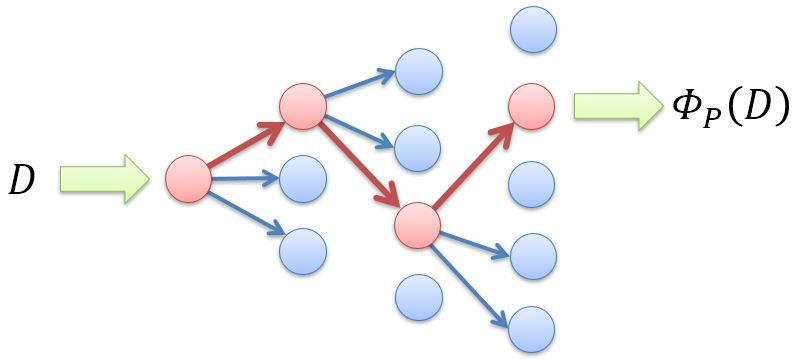
\includegraphics[width=1.0\textwidth]{figures/domainpath.jpg}
  \caption{} \label{fig:domainpath}
\end{subfigure}
\begin{subfigure}[b]{0.4\textwidth}
  \centering
  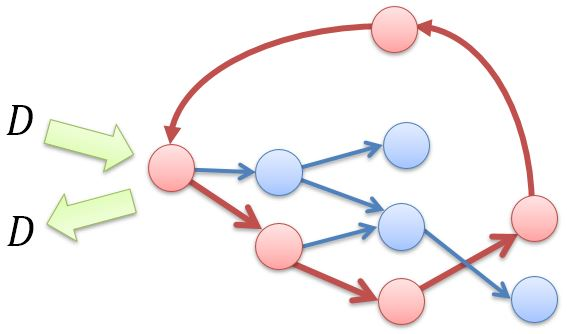
\includegraphics[width=0.8\textwidth]{figures/domaincycle.jpg}
  \caption{} \label{fig:domaincycle}
\end{subfigure}
\caption{Доменный путь (a) и доменный цикл (b)}
\end{figure}

Далее, предположим, что в графе $G$ нет доменных циклов.
Наличие доменных циклов говорит о наличии в сети \textit{бесконечных циклов маршрутизации} \cite{tanenbaum1996computer}.
То есть существует пакет, который будет следовать по одному и тому же пути в течение неопределенного промежутка времени.
Бесконечные циклы маршрутизации считаются ошибками настройки сети, так как они могут привести к более серьезным проблемам, таким как \textit{широковещательные штормы} \cite{tseng2002broadcast}.
Сетевые администраторы стремятся избавиться от подобных ошибок, поэтому существует множество методов обнаружения бесконечных циклов маршрутизации и удаления их из сети \cite{kazemian2012header,kazemian2013real,hengartner2002detection}.

Необхобимо отметить, что мы не предполагаем отсутствия в сети \textit{конечных циклов маршрутизации}, в которых пакеты в конечном итоге выйдут из цикла, например, циклов на уровне L2.

\begin{proposition} \label{th:domain_path_v_t}
$\forall v\in V$ и $\forall n\in D_v$ существует $n$-доменный путь $P_n:v=v_0,\dots,v_l=t$, где $t\in T$.
\end{proposition}

\begin{proof}
Покажем существование такого пути.
Зафиксируем произвольную вершину $v$ и произвольный элемент $n\in D_v$.
Опишем процедуру построения пути $P_n:v=v_0,\dots,v_l$.

Путь $P_n^0$, состоящий из одной вершины $v_0$, является доменным путем, так как $\Phi_{v_0}(n) = \{n\}$ и $\{n\}\subseteq D_{v_0}$.
Если $v_0\in T$, то теорема доказана.
Далее, предположим, что $v_0\notin T$.

Рассмотрим произвольный шаг с номером $i\geqslant 1$.
Пусть построен путь $P_n^i:v=v_0,\dots,v_i$ такой, что $\Phi_{v_0,\dots,v_{i-1}}(n)\subseteq D_{v_i}$.
Если $v_i\in T$, то теорема доказана, если нет, то предположим, что $v_i\notin T$.
Тогда из \eqref{eq:default_rule} следует, что существует ребро $v_iv_{i+1}$ такое, что $\Phi_{v_0,\dots,v_i}(n)\cap D_{v_iv_{i+1}}\neq \varnothing$.
И так как $D_{v_iv_{i+1}}\subseteq D_{v_{i+1}}$, то $\Phi_{v_0,\dots,v_i}(n)\cap D_{v_{i+1}}\neq \varnothing$ и $P_n^i$ --- $n$-доменный путь.

Пусть существует номер $j$ такой, что $v_j = v_i$ для некоторого $i<j$, то есть, вершина уже участвовала в пути $P_n$.
Если $\Phi_{v_0,\dots,v_i}(n) = \Phi_{v_0,\dots,v_j}(n)$, то в графе $G$ существует доменный цикл, что противоречит предположению об отсутствии доменных циклов.
Следовательно:
\begin{equation} \label{eq:domain_path_v_t_1}
    \Phi_{v_0,\dots,v_i}(n)\neq \Phi_{v_0,\dots,v_j}(n)\quad \forall i,j>0.
\end{equation}

Покажем, что $\forall j: v_j\notin T$ будет существовать шаг с номером $k>j$ такой, что вершина $v_k$ ранее не встречалась в пути $P$.
Пусть для некоторого $j$ такого номера не существует.
Так как на каждом шаге процедуры строится путь, проходящий через вершину, не являющуюся стоком, то по \eqref{eq:default_rule} получаем, что процедура будет иметь бесконечное число шагов.
Тогда существует хотя бы одна вершина $v_k$, которая участвует в бесконечном числе шагов описанной процедуры.
Но из конечности $D_{v_k}$ получаем, что существуют номера $k',k''>j$ такие, что $v_{k'} = v_{k''} = v_k$ и $\Phi_{v_0,\dots,v_{k'}}(n) = \Phi_{v_0,\dots,v_{k''}}(n)$.
Таким образом получено противоречие с \eqref{eq:domain_path_v_t_1}.

Следовательно, всегда существует шаг описанной процедуры такой, что вершина рассматриваемого шага ранее не участвовала в пути $P$.
И так как множество $V$ конечно, то из-за \eqref{eq:default_rule} описанная процедура может закончиться только в некоторой стоковой вершине $v_l\in T$.
Следовательно $P_n:v=v_0,\dots,v_l=t$ --- $n$-доменный путь из $v$ в $t$, и утверждение доказано.
\end{proof}

\begin{definition}
Пусть $v \in V \setminus S$.
Домен $n \in D_v$ называется \textit{достижимым}, если:
\begin{equation}
    \exists uv \in A : n \in D_{uv}.
\end{equation}
Множество достижимых доменов для вершины $v$ обозначим через $R_v \subseteq D_v$.
\end{definition}

\begin{definition}
\textit{Потоком} $D$-\textit{доменного пути} $P_D\in \mathscr{P}$ из вершины $v$ в вершину $w$ при $D\subseteq D_v$ назовем функцию $F:\mathscr{P}\rightarrow \mathbb{N}$, такую что:
\begin{equation} \label{eq:F(P_D)}
    F(P_D) = \sum_{n\in D} {f_n(v)},
\end{equation}
где $\mathscr{P}$ --- множество всех доменных путей в графе $G$.
\end{definition}

Поток $D$-доменного пути описывает количество пакетов с заголовками $h$ и входными портами $p$, такими что $(h,p)\in D$, которые вышли из вершины $v$ и двигались вдоль этого пути.

\begin{definition}
\textit{Подпространством доменных путей в вершину} $v$ назовем
\begin{equation}
    \mathcal{P}(v) = \{ P_n:u\rightarrow v \;|\; n \in\mathcal{N}, u\in S \}.
\end{equation}
\end{definition}

Введем следующее обозначение:
\begin{equation}
    F\big( \mathcal{P}(v) \big) = \sum_{P_n\in\mathcal{P}(v)}{F(P_n)}.
\end{equation}

\begin{theorem} \label{th:f_P_v}
Для любой вершины $v\in V$ графа верно:
\begin{equation}
    f(v) = F\big(\mathcal{P}(v)\big).
\end{equation}
\end{theorem}

\begin{proof}
Построим последовательность множеств $\mathcal{P}^i(v)$ различных доменных путей длины $i$ в вершину $v$, при $i \in [0,l]$, где $l$ --- длина максимального $n$-доменного пути для некоторого $n \in\mathcal{N}$.
Длина путей ограничена в силу предположения об отсутствии в графе доменных циклов.
\begin{equation}
    \mathcal{P}^i(v) = \mathcal{P}^i_R(v) \cup \mathcal{P}^i_S(v) \cup \mathcal{P}^i_U(v),
\end{equation}
где:
\begin{alignat}{4}
    \mathcal{P}^i_R(v) &= \{ P_n:u\rightarrow v \;&|&\; n\in D_u\cap R_v,           ~&&u\in V\setminus S, ~&|P_n| = i   &\}, \\
    \mathcal{P}^i_S(v) &= \{ P_n:u\rightarrow v \;&|&\; n\in D_u,                   ~&&u\in S,            ~&|P_n|\leqslant i &\}, \\
    \mathcal{P}^i_U(v) &= \{ P_n:u\rightarrow v \;&|&\; n\in D_u\cap\overline{R}_v, ~&&u\in V\setminus S, ~&|P_n|\leqslant i &\}.
\end{alignat}

$\mathcal{P}^i_R(v)$ и $\mathcal{P}^i_U(v)$ не пересекаются с $\mathcal{P}^i_S(v)$, так как пути $P_n$ начинаются из непересекающихся множеств вершин $S$ и $V\setminus S$.
$\mathcal{P}^i_R(v)$ не пересекается с $\mathcal{P}^i_U(v)$, так как пути $P_n$ начинаются из непересекающихся множеств доменов $D_u\cap R_v$ и $D_u\cap\overline{R}_v$.

Покажем, что $\forall i\in[0,l]$ выполняется:
\begin{equation} \label{eq:f_P_v_1}
    f(v) = F\big(\mathcal{P}^i(v)\big).
\end{equation}

\textit{База индукции} при $i=0$:  

Рассмотрим множество $\mathcal{P}^0(v)$.
Если $v\in S$, то получаем, что $\mathcal{P}^0(v) = \mathcal{P}^0_S(v)$.
Если $v\in V\setminus S$, то $\mathcal{P}^0(v) = \mathcal{P}^0_R(v) \cup \mathcal{P}^0_U(v)$.
$\mathcal{P}^0(v)$ по определению описывает множество всех $P_n:v\rightarrow v$ путей длины 0, при $n\in D_v$.

По определению потока доменного пути получаем, что $F(P_n) = f_n(v)$ для любого $P_n\in \mathcal{P}^0$.
Далее из определения потока через вершину и определения потока доменного пути получаем:
\begin{equation}
    f(v) = \sum_{n\in D_v}{f_n(v)} = \sum_{P_n\in \mathcal{P}^0(v)}{F(P_n)} = F\big(\mathcal{P}^0(v)\big).
\end{equation}

\textit{Шаг индукции}:

Пусть утверждение \eqref{eq:f_P_v_1} доказано для некоторого $k < l$, где $l$ --- длина максимального $n$-доменного пути для некоторого $n \in\mathcal{N}$. Поэтому докажем его для $k+1$.
Построим инъективное отображение $\varphi$ (рис. \ref{fig:relation}) из множества $\mathcal{P}^{k}(v)$ в множество $\mathcal{P}^{k+1}(v)$ такое, что:
\begin{equation}
    F(P) = \sum_{P^{'}\in \varphi(P)}{F(P')}.
\end{equation}

\begin{figure}
\centering
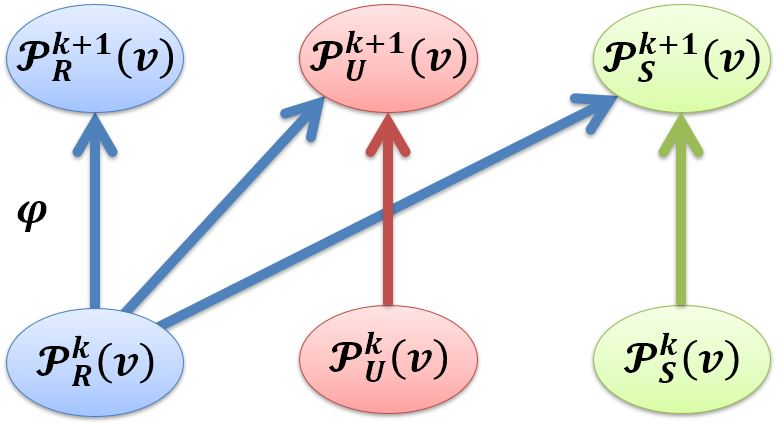
\includegraphics[width=0.4\textwidth]{figures/relation.jpg}
\caption{Инъективное отображение} \label{fig:relation}
\end{figure}

Инъективным отображением называется такое отображение $\varphi:\mathcal{P}^k(v) \rightarrow \mathcal{P}^{k+1}(v)$, что $\varphi(P)=\varphi(P')\Rightarrow P = P'$ для любых $P \in \mathcal{P}^k(v)$ и $P' \in \mathcal{P}^{k+1}(v)$.
Таким образом, если такое отображение существует, то будет доказано, что $F\big(\mathcal{P}^{k}(v)\big) = F\big(\mathcal{P}^{k+1}(v)\big)$.

Покажем, что каждому доменному пути $P\in \mathcal{P}^k_S(v)$ однозначно соответствует некоторый доменный путь $P'\in \mathcal{P}^{k+1}_S(v)$ такой, что $F(P) = F(P')$.
Утверждение очевидно, так как в данном случае $P = P'$, то есть один и тот же путь длины $k$ принадлежит обоим множествам.
Таким же образом доказывается, что каждому доменному пути $P\in \mathcal{P}^k_U(v)$ однозначно соответствует некоторый доменный путь из $P'\in \mathcal{P}^{k+1}_U(v)$.
Очевидно, что $\varphi\big(\mathcal{P}^k_S(v)\big) \neq \mathcal{P}^{k+1}_S(v)$ так как $\mathcal{P}^{k+1}_S(v)$ содержит еще и пути длины $k+1$.

Введем следующие обозначения:
\begin{align}
    \mathcal{P}'_S &= \mathcal{P}^{k+1}_S(v) \setminus \varphi\big( \mathcal{P}^{k}_S(v) \big), \\
    \mathcal{P}'_U &= \mathcal{P}^{k+1}_U(v) \setminus \varphi\big( \mathcal{P}^{k}_U(v) \big), \\
    \mathcal{P}'_R &= \mathcal{P}^{k+1}_R(v) \cup \mathcal{P}'_S \cup \mathcal{P}'_U.
\end{align}
Теперь построим инъекцию $\varphi: \mathcal{P}^{k}_R(v) \rightarrow \mathcal{P}'_R$.
Возьмем произвольный доменный путь $P_n\in \mathcal{P}^{k}_R(v)$ и рассмотрим начальную вершину $u$ этого пути.
Так как домен $n\in D_u$ достижим, то существует ребро $wu$ такое, что $n\in D_{wu}$.
Таким образом:
\begin{equation}
    F(P_n) = f_n(u) = \sum_{wu\in A}{\hat{f}_n(w,u)} = \sum_{wu\in A}{\ \sum_{m\in \Phi^{-1}_w(n)}{f_m(w)} }.
\end{equation}

Рассмотрим произвольный домен $m\in \Phi^{-1}_w(n)$.
Путь $wP_n$ является $m$-\linebreak доменным путем из $w$ в $v$, так как $m_w = \Phi_u(m) = n$, и $P_n$ --- $n$-доменный путь из $u$ в $v$.
Так как $wP_n$ --- $m$-доменный путь из $w$ в $v$, то $F(wP_n) = f_m(w)$.
Таким образом, получаем:
\begin{equation}
    F(P_n) = \sum_{wu\in A}{\ \sum_{m\in \Phi^{-1}_w(n)}{f_m(w)} } = \sum_{wu\in A}{\ \sum_{m\in \Phi^{-1}_w(n)}{F(wP_n)} } = \sum_{P_m\in \mathcal{P}'_R(v; P_n)}{F(P_m)},
\end{equation}
где $\mathcal{P}'_R(v; P_n) = \{ wP_n\ |\ wu\in A,\ m\in \Phi^{-1}_w(n) \}$ при $P_n:u\rightarrow v$ из множества $\mathcal{P}^{k}_R(v)$.

Поставим каждому доменному пути $P_n\in \mathcal{P}^k_R(v)$ набор путей $\varphi(P_n) = \mathcal{P}'_R(v; P_n)$, построенных по описанной выше процедуре. Получаем, что:
\begin{equation}
    F(P_n) = \sum_{P_m\in \varphi(P_n)}{F(P_m)}.
\end{equation}

Покажем, что $\varphi$ --- инъективное отображение из $\mathcal{P}^k_R(v)$ в $\mathcal{P}'_R$.
По построению следует, что $\forall P_n\in \mathcal{P}^k_R(v)$ существует некоторый $P_m = \varphi(P_n)$.
Покажем, что $\forall P_m$ существует единственный доменный путь $P_n = \varphi^{-1}(P_m)$, то есть для различных доменных путей $P_n$ и $P'_n$ множества $\mathcal{P}'_R(v; P_n)$ и $\mathcal{P}'_R(v; P'_n)$ не пересекаются.
Пусть существует путь $P_m$, принадлежащий обоим множествам. Но тогда $P_m = wP_n = wP'_n$, что противоречит различности $P_n$ и $P'_n$.

Теперь предположим, что $\exists P_m\in \mathcal{P}'_R$ такое, что $\nexists P_n\in \mathcal{P}^k_R(v):\ P_m = \varphi(P_n)$.
Так как все пути $P_m:u_1\dots u_kv\in \mathcal{P}'_R$ имеют длину $k+1$, то $P_n:u_2\dots u_kv$ имеет длину $k$.
Но тогда данный путь должен был быть выбран в описанной выше процедуре, которая бы построила непустое множество $\varphi(P_n)$.

Таким образом, доказано, что $\varphi: \mathcal{P}^{k}(v)\rightarrow \mathcal{P}^{k+1}(v)$ --- инъекция, и $F\big(\mathcal{P}^{k}(v)\big) = F\big(\mathcal{P}^{k+1}(v)\big)$, и индукция завершена.

Далее, из определения следует, что $\mathcal{P}(v) = \mathcal{P}^l_S(v)$, так как $l$ --- длина максимального доменного пути.
Покажем, что $\mathcal{P}^l_R(v) = \varnothing$.
Предположим противное.
Тогда существует путь $P_n\in \mathcal{P}^l_R(v)$ длины $l$ такой, что $n$ --- достижимый домен.
Следовательно, существует вершина $w$ такая, что $wP_n = P_m$ --- $m$-доменный путь длины $l+1$ для некоторого домена $m$, что противоречит максимальности $l$.
Также покажем, что $F\big(\mathcal{P}^l_U(v)\big) = 0$.
Это свойство следует из \eqref{eq:f_n(v)} и определения достижимого домена:
\begin{equation}
    F\big(\mathcal{P}^l_U(v)\big) = \sum_{P_n\in \mathcal{P}^l_U(v)} {F(P_n)} = \sum_{u\in V\setminus S} {\ \sum_{n\in D_u\cap\overline{R}_v} {f_n(u)}} = 0.
\end{equation}

Таким образом, получаем, что:
\begin{eqnarray}
    f(v) = F\big(\mathcal{P}^l(v)\big) = F\big(\mathcal{P}^l_S(v)\big) = F\big(\mathcal{P}(v)\big),
\end{eqnarray}
и теорема доказана.
\end{proof}

Рассмотрим множество $\mathcal{P}$.
Пусть $P$ --- произвольный путь из $S$ в $v$ в графе $G$.
Рассмотрим все доменные пути $P_n\in \mathcal{P}(v)$ такие, что $P_n$ и $P$ равны как пути в графе, то есть $E(P_n)=E(P)$.
Построим новый доменный путь из пути $P$, приписыванием к нему домена $D$, равного объединению всех доменов путей $P_n$ таких, что $E(P_n)=E(P)$.
Построим следующее множество:
\begin{equation}
    \mathbb{P}(v) = \bigg\{ P_D\ :\ D=\bigcup_{\substack{P_n\in \mathcal{P}(v) \\ E(P_n)=E(P)}}{D(P_n)} \bigg\}.
\end{equation}

Также определим поток по доменным путям $P_D\in \mathbb{P}(v)$ как:
\begin{equation}
    F(P_D) = \sum_{n\in D}{F(P_n)}.
\end{equation}

Из построения следует, что все пути из $\mathbb{P}(v)$ различны. Из доказанной выше теоремы следует, что:

\begin{corollary}
Для любой вершины $v \in V$ выполняется следующее:
\begin{equation}
    f(v) = F\big(\mathbb{P}(v)\big).
\end{equation}
\end{corollary}

Обозначим через $\mathbb{P}$ объединение пространств путей для всех вершин графа $G$, то есть:
\begin{equation}
    \mathbb{P} = \bigcup_{v\in V}{\mathbb{P}(v)}.
\end{equation}
Введем на множестве $\mathbb{P}$ отношение частичного порядка <<$\preceq$>>.

\begin{definition}
Пусть $P,P'\in \mathbb{P}$, тогда $P \preceq P'$ если:
\begin{enumerate}
\item $P$ и $P'$ имеют общую начальную вершину;
\item $E(P) \subseteq E(P')$.
\end{enumerate}
\end{definition}

Таким образом, $\mathbb{P}$ есть решетка путей в графе $G$.
Обозначим через $\mathbb{P}|_P$ подрешетку, образованную из всех путей $P'\in \mathbb{P}$ таких, что $P\preceq P'$.
Для путей $P\preceq P'$ определена операция <<$-$>> такая, что путь $P' - P$ получен из $E(P') \setminus E(P)$ удалением вершин с нулевой степенью.

\begin{definition}
Мультипликатором пути $P=v_0,\dots,v_k$ назовем следующую величину:
\begin{equation}
    \hat{\gamma}(P) = \prod_{i\in [0,k-1]} {\gamma(v_i)},
\end{equation}
где $\gamma(v)$ - степень дублирования вершины $v$.
Если $E(P) = \varnothing$, то $\hat{\gamma}(P) = 1$.
\end{definition}

\begin{theorem} \label{th:antichain}
\begin{equation} \label{eq:antichain}
    F(P) = \sum_{P'\in AC(P)} {\frac{F(P')}{\hat{\gamma}(P'\setminus P)}},
\end{equation}
где $AC(P)$ есть произвольная максимальная по включению антицепь из $\mathbb{P}|_P$.
\end{theorem}

\begin{proof}
Зафиксируем некоторую антицепь $AC(P)$ и проведем доказательство по индукции.
Построим последовательность множеств $\mathbb{P}^i =$\linebreak$\mathbb{P}^i_{AC}\cup \mathbb{P}^i_{=}$ при $i\in [0,l]$, где $l$ --- длина максимального по длине доменного пути.
\begin{alignat}{2}
    &\mathbb{P}^i_{AC} &\;=\;& \{P' : |P'|\leqslant i, P'\in AC(P)\}, \\
    &\mathbb{P}^i_{=}  &\;=\;& \{P' : |P'|  =  i, P'\in \mathbb{P}|_P, P'\prec AC(P)\},
\end{alignat}
где под $P'\prec AC(P)$ понимается, что существует элемент из антицепи $AC(P)$, который больше, чем $P'$.
Докажем, что:
\begin{equation} \label{eq:antichain_3}
    F(P) = \sum_{P'\in \mathbb{P}^l}{\frac{F(P')}{\hat{\gamma}(P'-P)}}.
\end{equation}

\textit{База индукции} при $i=0$:

База индукции выполняется, так как $P$ --- единственный элемент из $\mathbb{P}^0$ и $\hat{\gamma}(P-P)=1$, то есть:
\begin{equation}
    F(P) = \frac{F(P)}{\hat{\gamma}(P-P)}.
\end{equation}

\textit{Шаг индукции}:

Пусть \eqref{eq:antichain_3} выполнено для некоторого $i>0$.
Для перехода к $i+1$ поочередно рассмотрим все пути $P'\in \mathbb{P}^i_{=}$ и их концевые вершины $v$.
Если $\mathbb{P}^i_{=}$ непусто, то $v\notin T$, так как $\exists P''\in AC(P):\ P''\succ P'$, в то время как пути, оканчивающиеся в $T$, максимальные.

По определению путь $P'$ из $\mathbb{P}$ с концевой вершиной $v$ принадлежит множеству $\mathbb{P}(v)$ и раскладывается на доменные пути $P'_n$ такие, что $n\in D(P')$, где $D(P')$ --- домен пути $P'$.

Для любого пути $P'_n$ существует $\gamma(v)$ ребер $vw$ таких, что:
\begin{equation}
    \Phi_v\big(D_v(P'_n)\big)\cap D_{vw}\neq \varnothing,
\end{equation}
где $D_v(P'_n) = n_{P'}$.
Следовательно, существует $\gamma(v)$ доменных путей $P'_n w$ длины $i+1$ таких, что $F(P'_n)=F(P'_n w)$.
Это равенство выполняется, потому что потоки доменных путей равны $f_n(s)$, где $s$ --- общее начало обоих путей.

Следовательно, слагаемое $\frac{F(P')}{\hat{\gamma}(P'-P)}$ из \eqref{eq:antichain_3} для $i$ разлагается в сумму:
\begin{equation} \label{eq:antichain_4}
    \frac{F(P')}{\hat{\gamma}(P'-P)}
    = \frac{1}{\hat{\gamma}(P'-P)}
      \sum_{n\in D(P')}
      {
        \sum_{vw\in A}
        {
            I_n(vw) \frac{1}{\gamma(v)} F(P'_n w)
        }
      },
\end{equation}
\begin{equation}
    \text{где } I_n(vw) = 
    \begin{cases}
        1, & \text{if } \Phi_v\big(D_v(P'_n)\big)\cap D_{vw}\neq \varnothing, \\
        0, & \text{иначе}.
    \end{cases}
\end{equation}

Изменим порядок слагаемых в \eqref{eq:antichain_4}:
\begin{equation} \label{eq:antichain_5}
    \sum_{vw\in A}
    {
        \frac{1}{\hat{\gamma}(P'-P)} \frac{1}{\gamma(v)}
        \sum_{n\in D(P')} { I_n(vw) } F(P'_n w)
    }.
\end{equation}

Рассмотрим путь $P'' = P'w$ с доменом $D(P'')$:
\begin{equation}
    D(P'') = \big\{ n\in D(P')\ :\ I_n(vw)=1 \big\}.
\end{equation}
Путь $P''\in\mathbb{P}(w)$, так как $P''$ является объединением путей $P'_n w$ и не существует такого пути $P''_m\in \mathcal{P}(w)$, что $E(P'') = E(P''_m)$ и $m\notin D(P'')$.

Также из определения мультипликатора пути следует, что:
\begin{equation}
    \frac{1}{\hat{\gamma}(P'-P)} \frac{1}{\gamma(v)} = \frac{1}{\hat{\gamma}(P''-P)}.
\end{equation}

Остается показать, что каждый $P''$ принадлежит $\mathbb{P}^{i+1}$.
Это утверждение очевидно выполняется, если $P''\in AC(P)$, так как длина пути $P''$ есть $i+1$.

Пусть теперь $P''\notin AC(P)$.
Предположим, что $P''\notin \mathbb{P}^{i+1}_{=}$.
Так как $P''\in\mathbb{P}|_P$, то не существует $\hat{P}\in AC(P)$ такого, что $\hat{P} \succ P''$.
По построению множества $\mathbb{P}^{i+1}$ видно, что мы не могли построить путь такой, что $P'' \succ AC(P)$, так как процедура увеличения происходила только для путей из $\mathbb{P}^{i}_{=}$.
Таким образом, мы получили путь $P''$, не сравнимый ни с каким элементом антицепи $AC(P)$, что противоречит ее максимальности по включению.

Таким образом, каждое слагаемое $\frac{F(P')}{\hat{\gamma}(P'-P)}$ из \eqref{eq:antichain_3} для $i$ раскладывается в сумму $\sum{\frac{F(P'')}{\hat{\gamma}(P''-P)}}$, где каждый $P''\in \mathbb{P}^{i+1}$.

Для доказательства теоремы остается показать, что $\mathbb{P}^{l} = AC(P)$.
Для этого нужно показать, что $\mathbb{P}^{l}_{=} = \varnothing$.
Пусть существует $\overline{P}\in \mathbb{P}^{l}_{=}$.
Так как из утверждения \ref{th:domain_path_v_t} следует, что для каждой вершины $v$ и каждого $n\in D_v$ существует доменный путь в $T$, то любой путь $\overline{P}$ максимальной длины должен заканчиваться в $T$.
Что приводит к противоречию, так как $\nexists \overline{P}' \succ \overline{P}$, потому что пути, заканчивающиеся в $T$ --- максимальные элементы решетки $\mathbb{P}$.
\end{proof}

\begin{definition}
Антицепью называется такое подмножество $U$ частично-упорядоченного множества, что любая пара элементов $u, v\in U$ несравнима.
\end{definition}

Далее докажем следующее утверждение:

\begin{proposition}
$\mathbb{P}(T)$ есть максимальная по включению антицепь в $\mathbb{P}$.
\end{proposition}

\begin{proof}
Так как пути, заканчивающиеся в $T$ --- максимальные элементы решетки $\mathbb{P}$, то очевидно, что элементы из $\mathbb{P}(T)$ несравнимы, и $\mathbb{P}(T)$ --- антицепь.
Далее, предположим, что антицепь $\mathbb{P}(T)$ не максимальна.
Тогда существует путь $P\in \mathbb{P}\setminus \mathbb{P}(T)$ несравнимый с $\mathbb{P}(T)$.
Что невозможно, потому что из утверждения \ref{th:domain_path_v_t} следует, что для любой вершины и любого домена существует путь $\overline{P}$ из данной вершины в $T$, для которого очевидно, что $\overline{P} \succ P$.
\end{proof}

Необходимо отметить, что любое подмножество антицепи также является антицепью.

Из доказанных ранее утверждений следует основная теорема:

\begin{theorem} \label{th:flow_decomposition}
\begin{equation} \label{eq:flow_decomposition}
    f(v) = \sum_{P\in \mathbb{P}(v)}{ \sum_{P'\in \mathbb{P}(T)\cap \mathbb{P}|_P}{ \frac{F(P')}{\hat{\gamma}(P'-P)} } }.
\end{equation}
\end{theorem}

Из теоремы \ref{th:flow_decomposition} следует, что поток через каждую вершину можно однозначно предсказать (рис. \ref{fig:decomposition}), используя значения потоков по путям в $P_D\in \mathbb{P}(T)$, которые в свою очередь равны значениям потоков $f_D(s)$.

\begin{figure}
\centering
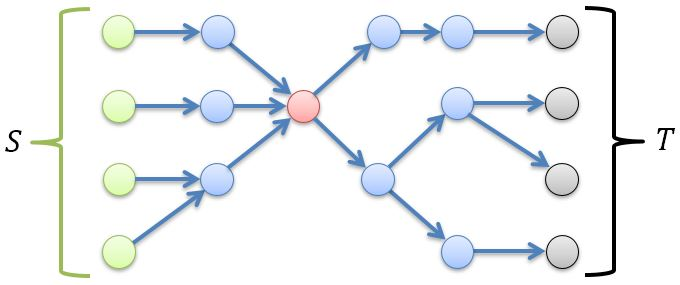
\includegraphics[width=0.6\textwidth]{figures/decomposition.jpg}
\caption{Предсказание потока через вершину} \label{fig:decomposition}
\end{figure}

Используем данный факт для построения алгоритма, который предсказывает значения потоков в вершинах по значениям потока в $S$.
Важно отметить, что в сумме \eqref{eq:flow_decomposition} один и тот же путь может встречаться несколько раз из-за возможности наличия в сети конечных циклов.

Докажем следующее утверждение:

\begin{proposition}
Пусть $P\in \mathbb{P}(T)$, тогда, если $\hat{\gamma}(P)=1$, то:
\begin{equation}
    \forall P'\in \mathbb{P}(T) : E(P')\neq E(P) \Rightarrow D(P)\cap D(P') = \varnothing.
\end{equation}
\end{proposition}

\begin{proof}
Предположим, что утверждение не выполняется. Тогда существует $n\in D(P)\cap D(P')$ при $E(P)\neq E(P')$.
Так как $\hat{\gamma}(P)=1$, то на каждой очередной вершине $v$ пути $P$, для любого $m\in D_v$ существует единственное ребро $vw$ такое, что $\Phi_v(m)\in D_{vw}$.
Таким образом, если $s$ --- начальная вершина пути $P$, то для любого $n\in D_s$ однозначно определен доменный путь $P_n$ такой, что $E(P)=E(P_n)=E(P')$, следовательно $n\in D(P)$.
Получено противоречие с тем, что $E(P)\neq E(P')$, и утверждение доказано.
\end{proof}

\subsection{Алгоритм предсказания потока}

Для построения алгоритма предсказания значений $f(v)$ определим граф $\mathcal{G}$, который назовем  \textit{путевой разверткой графа} $G$ (рис. \ref{fig:pathscan}).
Опишем алгоритм построения путевой развертки, представленный в алгоритме \ref{alg:create_path_scan}.

\begin{figure}
\centering
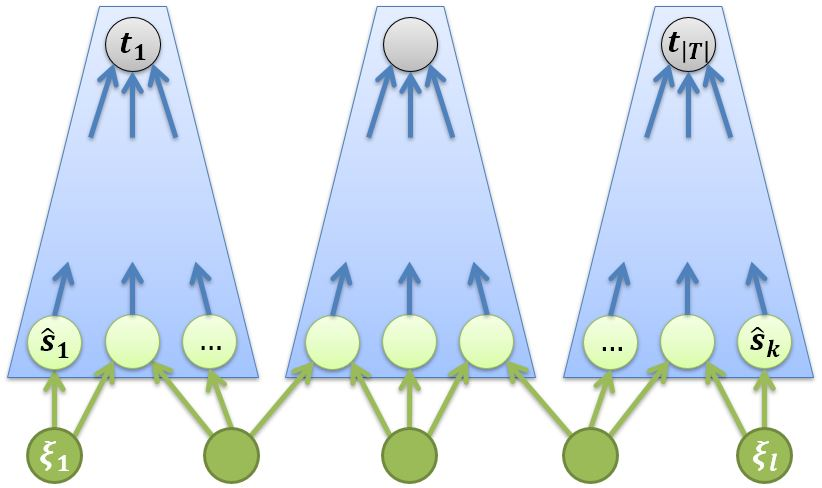
\includegraphics[width=0.6\textwidth]{figures/pathscan.jpg}
\caption{Путевая развертка} \label{fig:pathscan}
\end{figure}

Каждой вершине $v\in V$ соответствует множество вершин $\rho(v)\in \widetilde{V}$ в графе $\mathcal{G}$.
Каждой вершине $t\in T$ соответствует единственная вершина $\tilde{t} = \rho(t)$ с доменом $D_{\tilde{t}}= D_t$.
Множество таких вершин $\tilde{t}$, что $\rho^{-1}(\tilde{t})\in T$, будем обозначать как $\widetilde{T}$.

Зафиксируем некоторую вершину $\tilde{t}\in \widetilde{T}$ и опишем алгоритм построения дерева с корнем в $\tilde{t}$.
Занесем вершину $\tilde{t}$ в очередь $Q$.
Далее будем выбирать вершины из этой очереди до того, как она станет пустой.

Пусть на некотором шаге алгоритма из очереди была выбрана вершина $\tilde{v}$.
Для каждого ребра $uv\in A$, где $v = \rho^{-1}(\tilde{v})$, добавим в дерево вершину $\tilde{u}$ и ориентированное ребро $\tilde{u}\tilde{v}$.
Домены ребра $\tilde{u}\tilde{v}$ и вершины $\tilde{u}$ определим следующим образом:
\begin{alignat}{2}
    &D_{\tilde{u}\tilde{v}} &\;=\;& D_{uv}\cap D_{\tilde{v}}
    \label{eq:path_scan_arc_domain}, \\
    &D_{\tilde{u}} &\;=\;& \Phi^{-1}_u(D_{\tilde{u}\tilde{v}})
    \label{eq:path_scan_vertex_domain}.
\end{alignat}

Определим для вершины дерева $\tilde{u}$ значение $\hat{\gamma}(\tilde{u}) = \gamma(u)\hat{\gamma}(\tilde{v})$, где $\gamma(u)$ --- степень дублирования вершины $u$.
Значение $\hat{\gamma}(\tilde{u})$ назовем \textit{мультипликатором} вершины $\tilde{u}$.
Для вершин $\tilde{t}\in \widetilde{T}$ будем считать, что $\tilde{\gamma}(\tilde{t}) = 1$.

Далее занесем вершину $\tilde{u}$ в очередь $Q$ и продолжим выполнение алгоритма.
Алгоритм построения дерева закончится тогда, когда на некотором шаге из очереди будет удалена последняя вершина и не будет добавлена новая.

Удалим такие листовые вершины $\tilde{s}$ полученного дерева, что $\rho(\tilde{s})\notin S$ и перейдем к построению дерева с корнем $\tilde{t}'\in T\setminus{\tilde{t}}$.
Таким образом, мы построим дерево, соответствующее каждой вершине $t$ из множества $T$.
Множество всех вершин $\tilde{s}\in \rho^{-1}(s)$, где $s\in S$, обозначим как $\widetilde{S}$.

Выберем из построенных деревьев вершины $\tilde{s}\in \rho^{-1}(s)$, где $s\in S$, и построим разбиение $\mathscr{D}_s$ доменов $D_s$ такое, что:
\begin{equation}
    D_s = \bigsqcup_{D\in \mathscr{D}_s}{D},
\end{equation}
и для любого $\tilde{s}\in \rho^{-1}(s)$ существует $\widetilde{\mathscr{D}}_s\subseteq \mathscr{D}_s$ такое, что:
\begin{equation}
    D_{\tilde{s}} = \bigsqcup_{\widetilde{D}\in \widetilde{\mathscr{D}}_s} {\widetilde{D}}.
\end{equation}
Это разбиение можно построить, производя всевозможные пересечения доменов вершин $\tilde{s}\in \rho^{-1}(s)$.

Для каждого домена $D\in \mathscr{D}_s$ добавим в $\widetilde{V}$ вершину $\xi$ с доменом $D_{\xi} = D$.
Из вершины $\xi$ проведем ребро в вершину $\tilde{s}$ такую, что $\rho(\tilde{s})\in S$, и поставим ему в соответствие домен, равный $D_{\xi}$.
Множество всех таких $\xi$ обозначим за $\mathscr{S}$ и назовем \textit{множеством дополнительных вершин}.
На этом построение путевой развертки графа $G$ завершено.

\begin{figure}
\centering
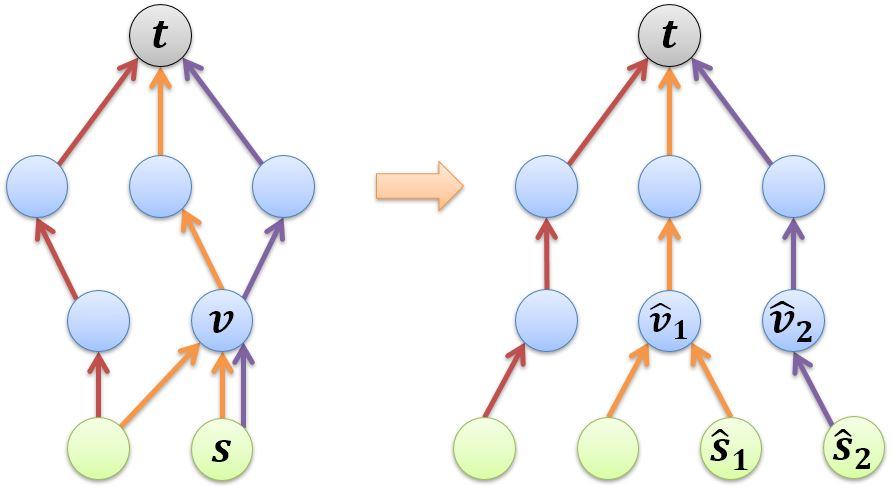
\includegraphics[width=0.6\textwidth]{figures/pathscancreation.jpg}
\caption{Построение путевой развертки} \label{fig:pathscancreation}
\end{figure}

Алгоритм \ref{alg:create_path_scan} также использует следующие дополнительные функции:
\begin{itemize}
    \item $create\_node(v, D, \gamma)$;
    \item $prune\_branch(\tilde{v})$;
    \item $create\_domain\_partition\big(\widetilde{S}\big)$.
\end{itemize}


Функция $create\_node(v, D, \gamma)$ создает новую вершину $\widetilde{v}$ путевой развертки, соответствующую вершине $v$ графа зависимостей правил.
В качестве домена вершины $\tilde{v}$ выбирается $D$, а в качестве мультипликатора --- $\gamma$, то есть:
\begin{alignat}{2}
    &D_{\widetilde{v}} = D, \\
    &\hat{\gamma}(\tilde{v}) = \gamma.
\end{alignat}
Функция $prune\_branch(\tilde{v})$ удаляет ветвь дерева путевой развертки, оканчивающуюся в вершине $\tilde{v}$.
Функция $create\_domain\_partition(\widetilde{S})$ создает набор новых вершин $\mathscr{S}$, доменами которых являются все попарные пересечения доменов вершин из $\widetilde{S}$.
То есть, создаются вершины с множеством доменов $\mathscr{D}_s$.
\\

Теперь опишем алгоритм предсказания значений $f(v)$, использующий путевую развертку.
Формальное описание представлено в алгоритме \ref{alg:flow_propagation}.
В этом алгоритме используются следующие обозначения: $\delta^{out}(\tilde{v})$ обозначает исходящие ребра из вершины $\tilde{v}$, а $\delta^{in}(\tilde{v})$ --- ребра, входящие в вершину $\tilde{v}$.

Предположим, что для любой вершины $\xi\in \mathscr{S}$ известны значения потоков $f(\xi)$.
Утверждается, что используя эту информацию можно предсказать значения потока $f(v)$ в каждой вершине $v\in V$.

Добавим в очередь $Q$ все вершины $\xi\in \mathscr{S}$ и припишем им значения потока $f(\xi)$.
Далее будем выбирать вершину $\tilde{v}$ из очереди $Q$ и добавлять значение ее потока $f(\tilde{v})$, деленное на $\hat{\gamma}(\tilde{w})$, в вершину $\tilde{w}$ такую, что она является родительской вершиной для $\tilde{v}$ в путевой развертке.
Ребро $\tilde{v}\tilde{w}$ отметим как просмотренное.

Если на очередном шаге все исходящие ребра некоторой вершины $\tilde{w}$ просмотрены, то добавляем вершину $\tilde{w}$ в очередь.
Алгоритм заканчивает свою работу, когда очередь $Q$ пуста.

Утверждается, что сумма значений $f(\tilde{v})$ по всем $\tilde{v}\in \rho^{-1}(v)$ есть поток $f(v)$.
Этот факт был доказан в теореме \ref{th:flow_propagation}.
\\

\begin{algorithm}
\caption{Построение путевой развертки} \label{alg:create_path_scan}
\hspace*{\algorithmicindent} \\
\hspace*{\algorithmicindent} \textbf{Input:} Граф зависимостей правил $G$ \\
\hspace*{\algorithmicindent} \textbf{Output:} Путевая развертка $\mathcal{G}(\widetilde{V}, \widetilde{A}, \mathscr{S})$
\begin{algorithmic}[1]
\Procedure{Create\_Path\_Scan}{$G$}
\For{$t\in T$}
    \State $\tilde{t}\gets\ $\textbf{create\_node}$(t, \mathcal{N}, 1)$
    \State $\widetilde{V}\gets \widetilde{V}\cup \{\tilde{t}\}$
    \State $Q\gets \tilde{t}$
\EndFor
\While{$Q\neq \varnothing$} \label{alg:create_path_scan:main_loop_begin}
    \State $\tilde{v}\gets Q$
    \State $v\gets \rho(\tilde{v})$
    \For{$u\in \delta^{in}(v)\ $\textbf{and}$\ D_{uv}\cap D_{\tilde{v}}\neq \varnothing$}
        \If{$\delta^{in}(u) = \varnothing\ $\textbf{and}$\ u\notin S$}
            \State \textbf{prune\_branch}$(\tilde{v})$
        \Else
            \State $D\gets \Phi^{-1}_{u}(D_{uv}\cap D_{\tilde{v}})$
            \State $\gamma\gets \gamma(u)\hat{\gamma}(\tilde{v})$
            \State $\tilde{u}\gets\ $\textbf{create\_node}$(u,D,\gamma)$
            \State $\widetilde{V}\gets \widetilde{V}\cup \{\tilde{u}\}$
            \State $\widetilde{A}\gets \widetilde{A}\cup \{\tilde{u}\tilde{v}\}$
            
            \If{$u\in S$}
                \State $\widetilde{S}\gets \tilde{u}$
            \Else
                \State $Q\gets \tilde{u}$
            \EndIf
        \EndIf
    \EndFor
\EndWhile \label{alg:create_path_scan:main_loop_end}
\State $\mathscr{S}\gets\ $ \textbf{create\_domain\_partition}$(\widetilde{S})$ \label{alg:create_path_scan:create_domain_partition}
\State \textbf{return}$\ \mathcal{G}(\widetilde{V}, \widetilde{A}, \mathscr{S})$
\EndProcedure
\end{algorithmic}
\end{algorithm}

\begin{algorithm}
\caption{Предсказание потока} \label{alg:flow_propagation}
\hspace*{\algorithmicindent} \\
\hspace*{\algorithmicindent} \textbf{Input:} Путевая развертка $\mathcal{G}(\widetilde{V}, \widetilde{A}, \mathscr{S})$ \\
\hspace*{\algorithmicindent} \textbf{Output:} Значение $f(v)$ для всех вершин $v\in V$
\begin{algorithmic}[1]
\Procedure{Predict\_Flow}{$\mathcal{G}$}
\For{$\xi\in \mathscr{S}$}
    \State $Q\gets \xi$
\EndFor

\While{$Q\neq \varnothing$} \label{alg:flow_propagation:main_loop_begin}
    \State $\tilde{v}\gets Q$
    \State $v\gets \rho^{-1}(\tilde{v})$
    \State $f(v)\gets f(v) + f(\tilde{v}) / \hat{\gamma}(\tilde{v})$
    
    \For{$\tilde{w}\in \delta^{out}(\tilde{v})$}
        \State $f(\tilde{w})\gets f(\tilde{w}) + f(\tilde{v})$
        \State $visited\gets visited\cup \{\tilde{w}\}$
        
        \If{$\delta^{in}(\tilde{w})\subseteq visited$}
            \State $Q\gets \tilde{w}$
        \EndIf
    \EndFor
\EndWhile \label{alg:flow_propagation:main_loop_end}
\State \textbf{return}$\ f$
\EndProcedure
\end{algorithmic}
\end{algorithm}

Введем следующее обозначение:
\begin{equation}
    \widetilde{\mathbb{P}}(v)
     = \Big\{ P_{\widetilde{D}}
         : s\rightarrow v\ 
       |\ 
         \widetilde{D} = D_{\tilde{s}}:\ 
         \tilde{s}\in \widetilde{S};\ 
         \exists \tilde{P}: \tilde{s}\rightarrow \tilde{v},\ 
         \tilde{v}\in \rho^{-1}(v)
       \Big\}.
\end{equation}
Докажем следующее утверждение:

\begin{proposition} \label{th:path_scan_at_vertex}
Для любого $t\in T$ следует, что:
\begin{equation}
    \widetilde{\mathbb{P}}(t) = \mathbb{P}(t).
\end{equation}
\end{proposition}

\begin{proof}
Докажем, что $\widetilde{\mathbb{P}}(t)\subseteq \mathbb{P}(t)$.
Пусть $P_{\widetilde{D}}=v_0,\dots,v_l\in \widetilde{\mathbb{P}}(t)$, где $v_0=s$ и $v_l=t$.
Покажем, что для любого $n\in \widetilde{D}$ $P_n$ является доменным путем для $n$.
Для этого проверим выполнение свойств доменного пути.
Из определения $\widetilde{\mathbb{P}}(t)$ следует, что $n\in D_{v_0}$. Из построения путевой развертки следует, что:
\begin{equation} \label{eq:path_scan_at_vertex_1}
    D_{\tilde{v}_{i-1}} = \Phi^{-1}_{v_{i-1}}(D_{v_{i-1}v_i}\cap D_{\tilde{v}_i}),
\end{equation}
и что $D_{\tilde{v}_i}\neq \varnothing$.
Таким образом, $n_{v_0,\dots,v_i}\neq \varnothing$.

Более того, из \eqref{eq:path_scan_at_vertex_1} следует, что не существует $m\notin \widetilde{D}$ такого, что $P_m$ является доменным путем, так как для вершины $v_{i+1}$ в каждом шаге алгоритма выбираются все возможные домены $m'\in D_{v_i}$, такие что $m'_{v_i}\cap D_{v_{i+1}}\neq \varnothing$.
Следовательно, $P_{\widetilde{D}}$ является объединением всех доменных путей из $s$ в $t$, то есть $P_{\widetilde{D}}\in \mathbb{P}(t)$.
Из чего следует, что $\widetilde{\mathbb{P}}(t)\subseteq \mathbb{P}(t)$.

Теперь докажем, что $\widetilde{\mathbb{P}}(t)\supseteq \mathbb{P}(t)$.
Возьмем произвольный путь $P=v_0,\dots,v_l\in \mathbb{P}(t)$.
По построению путевой развертки (алгоритм \ref{alg:create_path_scan}) существует путь  $\widetilde{P}\in \widetilde{\mathbb{P}}(t)$ такой, что $E(P)=E(\widetilde{P})$, то есть множество ребер путей совпадает.
Равенство доменов этих путей будет следовать из \eqref{eq:path_scan_at_vertex_1}.

Таким образом, доказано, что $\widetilde{\mathbb{P}}(t) = \mathbb{P}(t)$.
\end{proof}

Введем следующее обозначение: пусть $P\in \mathbb{P}(v)$ тогда:
\begin{equation}
    \widetilde{\mathbb{P}}|_P = \big\{ P'\in \widetilde{\mathbb{P}}(T)\ |\ E(P)\subseteq E(P') \big\}.
\end{equation}
Из утверждения \ref{th:path_scan_at_vertex} следует:

\begin{corollary} \label{th:path_scan_projection}
\begin{equation}
    \widetilde{\mathbb{P}}|_P = \mathbb{P}|_P\cap \mathbb{P}(T).
\end{equation}
\end{corollary}
\ \\
\ \\

Докажем основное утверждение:

\begin{theorem} \label{th:flow_propagation}
Для любой вершины $v\in V$ графа выполняется:
\begin{equation}
    \tilde{f}(v) = f(v),
\end{equation}
где $\tilde{f}(v)$ --- значение полученное алгоритмом \ref{alg:flow_propagation}.
\end{theorem}

\begin{proof}
Зафиксируем некоторую вершину $v\in V$.
Пусть $\tilde{f}(v)$ --- значение потока, которое приписывает алгоритм вершине $v$. Докажем, что $\tilde{f}(v)=f(v)$.
По построению алгоритма видно, что:
\begin{equation} \label{eq:flow_propagation_1}
    \tilde{f}(v) =
    \sum_{\tilde{v}\in \rho^{-1}(v)} {
        \sum_{P'\in \mathcal{I}(\tilde{v})} {
            \frac{F(P')}{\gamma(\tilde{v})}
        }
    },
\end{equation}
где:
\begin{equation}
    \mathcal{I}(\tilde{v}) = \big\{P'\in \widetilde{\mathbb{P}}(T)\ |\ \rho(\tilde{v})\in P'\big\}.
\end{equation}
То есть, значение потока в вершине $v$ складывается из значений потоков всех путей в путевой развертке, проходящих через вершины $\tilde{v}$ такие, что $\rho(\tilde{v}) = v$.

Каждый путь $P':s\rightarrow t$ в некотором слагаемом суммы \eqref{eq:flow_propagation_1} образует путь $P:s\rightarrow \rho(\tilde{v})$ такой, что $E(P)\subseteq E(P')$.
Стоит отметить, что, если вершина $v$ встречается в пути $P'$ несколько раз, то столько же путей будет образовано после перегруппироваки.
Также стоит отметить, что по построению $\gamma(\tilde{v})=\hat{\gamma}(P'-P)$.
Таким образом, слагаемые в сумме  \eqref{eq:flow_propagation_1} возможно перегруппировать следующим образом:
\begin{equation} \label{eq:flow_propagation_2}
\tilde{f}(v) = 
    \sum_{P\in \mathcal{J}(v)} {
        \sum_{P'\in \widetilde{\mathbb{P}}|_P} {
            \frac{F(P')}{\hat{\gamma}(P'-P)}
        }
    },
\end{equation}
где:
\begin{equation}
    \mathcal{J}(v) = \big\{P: S\rightarrow v\ | \ \exists P''\in \widetilde{\mathbb{P}}\ : \ E(P'')=E(P)\big\}.
\end{equation}

Из построения видно, что в сумме \eqref{eq:flow_propagation_2} не участвуют пути $P$ такие, что не существует $n$ таких, что $P_n$ не является доменным путем.
Поэтому пути в первой сумме принадлежат $\mathbb{P}(v)$, то есть $\mathcal{J}(v) = \mathbb{P}(v)$.
Таким образом, из следствия \ref{th:path_scan_projection} и теоремы \ref{th:flow_decomposition} следует:
\begin{equation}
\tilde{f}(v) = 
    \sum_{P\in \mathbb{P}(v)}{
        \sum_{
            P'\in \mathbb{P}(T)\cap \mathbb{P}|_P
        }{
            \frac{F(P')}{\hat{\gamma}(P'-P)}
        }
    } = 
f(v),
\end{equation}
и теорема доказана.
\end{proof}

Из теоремы \ref{th:flow_propagation} следует, что с помощью описанных выше алгоритмов возможно предсказать значения потока во всем графе зависимостей правил, зная значения потока на множестве $\mathscr{S}$, где $\mathscr{S}$ --- множество дополнительных вершин.
Это множество далее будет использоваться для создания дополнительных правил маршрутизации в сети.

\begin{proposition} \label{th:complexity}
Сложность алгоритма \ref{alg:create_path_scan} составляет $O(|V|*|\mathbb{P}| + |\mathbb{P}|^2)$, где $V$ --- множество вершин графа, $\mathbb{P}$ --- множество доменных путей в графе.
\end{proposition}

\begin{proof}
Строки \ref{alg:create_path_scan:main_loop_begin}---\ref{alg:create_path_scan:main_loop_end} описывают основной цикл алгоритма, который проходит по всем вершинам графа.
Из утверждения \ref{th:path_scan_at_vertex} следует, что алгоритм проходит по всем доменным путям графа.
Так как длина каждого доменного пути может быть ограничена сверху размером множества вершин, мы получаем сложность цикла, равную $O(|V|*|\mathbb{P}|)$.

Строка \ref{alg:create_path_scan:create_domain_partition} описывает вызов подпроцедуры, которая находит всевозможные пересечения пар доменов путей.
Так как в подпроцеуре производятся попарные пересечения доменов, то сложность подпроцедуры равна $O(|\mathbb{P}|^2)$.

Таким образом, получаем сложность алгоритма \ref{alg:create_path_scan}, равную\linebreak $O(|V|*|\mathbb{P}| + |\mathbb{P}|^2)$.
\end{proof}

\begin{proposition}
Сложность алгоритма \ref{alg:flow_propagation} составляет $O(|V|*|\mathbb{P}|)$, где $V$ --- множество вершин графа, $\mathbb{P}$ --- множество доменных путей в графе.
\end{proposition}

\begin{proof}
Строки \ref{alg:flow_propagation:main_loop_begin}---\ref{alg:flow_propagation:main_loop_end} описывают основной цикл алгоритма, который также, как и основной цикл алгоритма \ref{th:path_scan_at_vertex}, проходит по всем вершинам графа.
Таким образом, аналогично доказательству утверждения \ref{th:complexity} получаем сложность алгоритма \ref{alg:flow_propagation}, равную  $O(|V|*|\mathbb{P}|)$.
\end{proof}

Стоит отметить, что, если любой путь в графе зависимостей правил является доменным путем, то величина $|\mathbb{P}|$ может экспоненциально зависеть от количества вершин графа \cite{diestel2018graph}.
Но такая ситуация не описывает реальных механизмов маршрутизации, которые используются в ПКС \cite{kreutz2015software}.
Таким образом, реальное время работы алгоритма должно быть исследовано экспериментальным путем.

\begin{comment}
The complexity of NetPlumber for the addition of a single rule is O(r + spd), where r is the number of entries in each table and s is the number of source (sink) nodes attached to the plumbing graph (which is roughly proportional to the number of policies we want to check), p is the number of pipes to and from the rule and d is the diameter of the network.

Но необходимо отметить, что граф зависимостей правил может изменяться в ходе работы сети. Например, в сеть может быть установлено новое правило. После создания данного правила добавится новая вершина $v$ и добавятся новые ребра, ведущие к данному правилу. Также необходимо отметить, что правила $u$ в той же таблице, что и правило $v$, имеющие более низкий приоритет изменят свои домены на $D_u\setminus D_v$. 

Подобные изменения графа очевидно изменят $\mathbb{P}(T)$, поэтому необходимо производить перестроение путевой развертки. Так как изменения сети не обязательно будут влиять на все пути из $\mathbb{P}(T)$, то не нужно перестраивать заново всю развертку путей графа, вместо этого необходим алгоритм, который будет перестраивать только те пути, на которые повлияло изменение сети.

Также необходимо отметить, что за время между обновлениями сети по сети могло пройти некоторое количество пакетов, и значения счетчиков могли быть изменены. Поэтому необходимо, чтобы алгоритм обновления путевой развертки также сохранял данные значения счетчиков, для того, чтобы сохранять их консистентность после перестроения.

Граф зависимостей правил поддерживает возможность обработки изменения состояния сети [??]. Поддерживаются следующие изменения:
\begin{itemize}
\item Добавление правила
\item Удаление правила
\item Добавления сетевой линии
\item Удаление сетевой линии
\item Добавление таблицы
\item Удаление таблицы
\end{itemize}

После подобных изменений производится частичное (локальное) перестроение графа зависимостей. Например, после добавления правила производится добавление ребер графа и изменение доменов правил имеющий более низкий приоритет, чем новое. Также стоит отметить, что добавление/удаление таблицы эмулируется предыдущими 4мя изменениями сети.

Опишем добавление/удаление правил более формально. Пусть производится добавление (удаление) некоторой вершины $v$ в некоторую таблицу графа $G$. Обозначим через $C(v)$ множество вершин $u$ принадлежащих той же таблице, что и $v$, и имеющих более низкий приоритет, то есть $pr(u)<pr(v)$.

\begin{definition}
Добавлением вершины $v'$ в граф $G$, назовем отображение графа $G$ в граф $G'=G+v'$ такое, что:
\begin{enumerate}
\item Граф $G'$ также является графом зависимостей правил, то есть добавлены новые ребра $v'w$ по процедуре построения графа зависимостей правил
\item Для каждой вершины $v\in C(v)$ из доменов вершины $v$ и каждого ребра $uv$ выполняется $D'_v=D_v\setminus D_{v'}$, $D'_{uv}=D_{uv}\setminus D_{v'}$ и добавляется новое ребро $uv'$ такое, что $D_{uv'}=D_{uv}\cap D_{v'}$.
\end{enumerate}
\end{definition}

\begin{definition}
Удалением вершины $v'$ из графа $G$, назовем отображение графа $G$ в граф $G'=G-v'$ такое, что:
\begin{enumerate}
\item Из графа $G$ были удалены все ребра $uv'$ и $v'w$
\item Для каждой вершины $v\in C(v)$ из доменов вершины $v$ и каждого ребра $uv$ выполняется $D'_v=D_v\setminus D_{v'}$, $D'_{uv}=D_{uv}\setminus D_{v'}$ и добавляется новое ребро $uv'$ такое, что $D_{uv'}=D_{uv}\cap D_{v'}$.
\end{enumerate}
\end{definition}

\section{Модель атакующего}

\end{comment}

\end{document}